\documentclass[a4paper,12pt,oneside,final,spanish]{article}
%titlepage: pone el título en una página aparte
%twocolumn
\usepackage{babel} %Para el lenguaje [spanish]
\usepackage[utf8]{inputenc} %Para reconocer todos los símbolos
\usepackage[T1]{fontenc}
\usepackage{textcomp}
\usepackage{amsmath}
\usepackage{amsfonts}
\usepackage{amssymb}
\usepackage[margin=1.5cm]{geometry} %Márgenes
\usepackage[T1]{fontenc}
\usepackage{graphicx}
\usepackage{enumerate}
\usepackage{hyperref}
%\pagestyle{headings}

\title{\Huge Tecnologías para la Web Semántica\\
Trabajo Práctico Nº3\\
Metadatos}
\author{Darién Julián Ramírez}
\date{\vspace{-5ex}}

\begin{document}

\maketitle %Crea la página de título

\section*{Ejercicio 1}

Realice los siguientes pasos:

\begin{enumerate}[a.]
\item Cree un archivo html conteniendo una definición de Web Semántica y una breve descripción de sus características. (ws.htm) 
\item Utilice el estándar DC para su descripción:\\
\url{http://www.dublincore.org}\\
Aclaración: Puede utilizar el generador de metadatos siguiente:\\
\url{http://www.webposible.com/utilidades/dublincore-metadata-gen/index.php?lang=es}
\item Abra ws.htm. Posicione el cursor entre las etiquetas \textbf{<head>} y \textbf{</head>} y pegue los metadatos. Guarde el archivo. 
\item Abra ws.htm con Internet Explorer o cualquier otro navegador y examine los resultados.

\begin{quote}
No se observa ningún cambio, nada aparece.
\end{quote}

\item Inserte los micro formatos DC entre las etiquetas \textbf{<body>} y \textbf{</body>}.
\item Abra ws.htm con Internet Explorer o cualquier otro navegador y examine los resultados.

\begin{quote}
Se puede observar la información suministrada por las etiquetas.
\end{quote}

\item Explique la diferencia entre los resultados obtenidos en inciso d. y en inciso f. Guarde en el informe imágenes de los resultados.  

\begin{quote}
En el inciso d. la información mostrada está optimizada para ser útil a los buscadores miestras que en el inciso f. la información está optimizada para que sea útil para las personas.
\end{quote}

\begin{center}
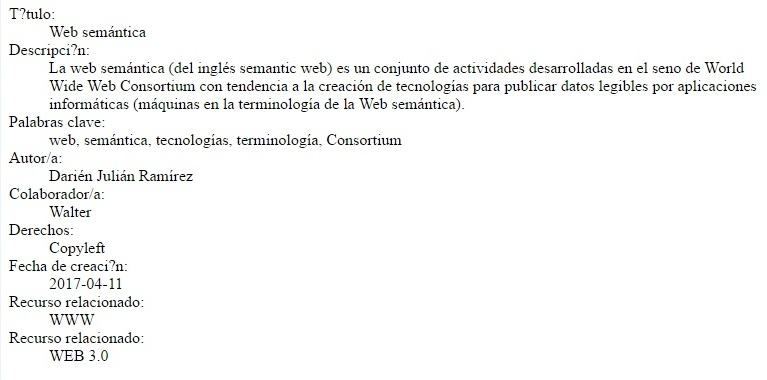
\includegraphics[width=0.9\linewidth,keepaspectratio]{wshtm}
\end{center}
\end{enumerate}

\section*{Ejercicio 2}

Investigue y responda:

\begin{enumerate}[a.]
\item ¿Qué es un Repositorio Institucional de Acceso Abierto? Explique.

\begin{quote}
El Acceso abierto es un movimiento que promueve el acceso libre y gratuito a la literatura científica, fomentando su libre disponibilidad en Internet y permitiendo a cualquier usuario su lectura, descarga, copia, impresión, distribución o cualquier otro uso legal de la misma, sin ninguna barrera financiera, técnica o de cualquier tipo. La única restricción sobre la distribución y reproducción es dar al autor el control sobre la integridad de su trabajo y el derecho a ser adecuadamente reconocido y citado.
El principal objetivo del acceso abierto es aumentar el impacto de la investigación al incrementar el acceso a la misma.
\end{quote}

\item ¿Qué es un Objeto de Aprendizaje?

\begin{quote}
Un objeto de aprendizaje es un conjunto de contenidos, ejercicios y elementos de evaluación que se combinan en relación a un único objetivo de aprendizaje. El término se atribuye a Wayne Hodgins y data de un grupo de trabajo que en 1994 llevaba ese nombre, aunque el concepto fue descrito por primera vez por Gerard en 1967.
\end{quote}

\item Considerando el apunte <<Metadatos>> como un objeto de aprendizaje realice las descripciones necesarias para su correcta localización y recuperación en un Repositorio Institucional de Acceso Abierto en FICH. Considere para ello un estándar de metadatos para objetos de aprendizaje.

\begin{quote}
Title: Metadatos.\\
Creator: Ing. Lucila Romero.\\
Subject: Metadatos.\\
Description: Descripciones y usos de los distintos tipos de metadatos.\\
Publisher: FICH.\\
Type: Informática.\\ 
Format:  Digital. \\
Language: Español. 
\end{quote}

\item ¿Qué modificaciones realizaría si se tratara de la descripción del trabajo práctico Metadatos? 

\begin{quote}
Title: Trabajo Práctico Metadatos.\\
Creator: Ing. Lucila Romero.\\
Subject: Metadatos.\\
Description: Ejercicios de introducción al manejo de metadatos.\\
Publisher: FICH.\\
Type: Informática.\\ 
Format: Digital. \\
Language: Español. 
\end{quote}

\end{enumerate}

\begin{thebibliography}{1}
\bibitem{AM2008}
Romero L.,
\emph{Apuntes de metadatos},
2008.

\bibitem{MC}
\emph{Material de clases}.

\bibitem{DC}
\emph{Guía para la creación de metadatos usando Dublín Core}.

\bibitem{DC}
\emph{IEEE LOM Standard}.
\end{thebibliography}

\end{document}